\documentclass{standalone}
\usepackage{tikz}
\usetikzlibrary{patterns, positioning}


\begin{document}
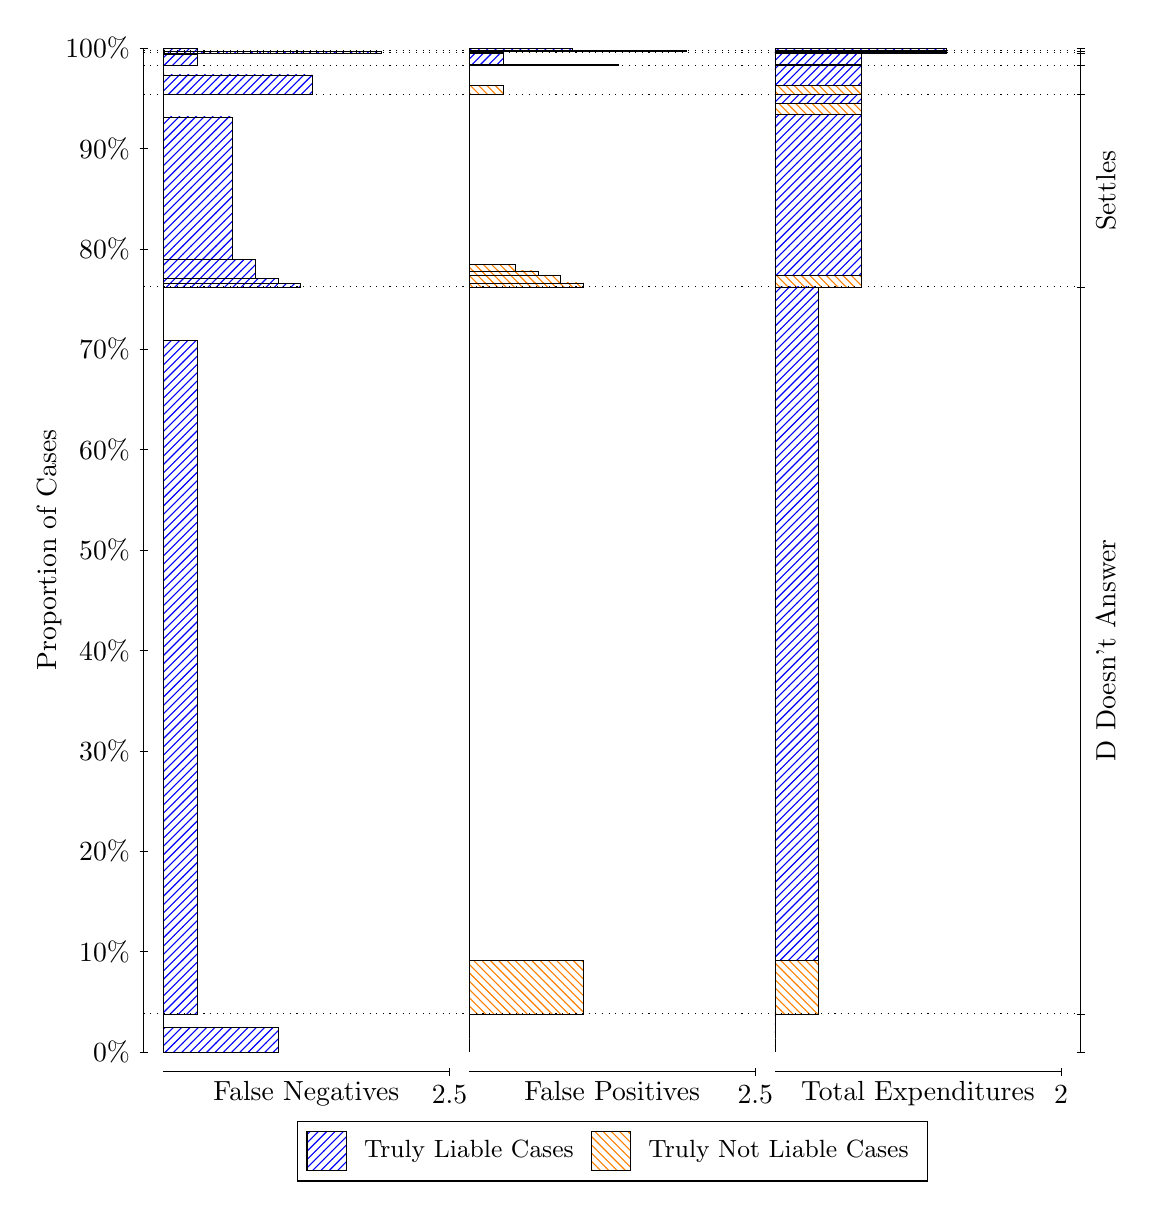
\begin{tikzpicture}
\draw[black, very thin] (1.5,1.75) -- (1.5,14.5);
\node[rotate=90, text=black, anchor=center] at (0.3, 8.125) {Proportion of Cases};
\draw[black, very thin] (1.45,1.75) -- (1.55,1.75);
\node[text=black, anchor=east] at (1.45, 1.75) {0\%};
\draw[black, very thin] (1.45,3.025) -- (1.55,3.025);
\node[text=black, anchor=east] at (1.45, 3.025) {10\%};
\draw[black, very thin] (1.45,4.3) -- (1.55,4.3);
\node[text=black, anchor=east] at (1.45, 4.3) {20\%};
\draw[black, very thin] (1.45,5.575) -- (1.55,5.575);
\node[text=black, anchor=east] at (1.45, 5.575) {30\%};
\draw[black, very thin] (1.45,6.85) -- (1.55,6.85);
\node[text=black, anchor=east] at (1.45, 6.85) {40\%};
\draw[black, very thin] (1.45,8.125) -- (1.55,8.125);
\node[text=black, anchor=east] at (1.45, 8.125) {50\%};
\draw[black, very thin] (1.45,9.4) -- (1.55,9.4);
\node[text=black, anchor=east] at (1.45, 9.4) {60\%};
\draw[black, very thin] (1.45,10.675) -- (1.55,10.675);
\node[text=black, anchor=east] at (1.45, 10.675) {70\%};
\draw[black, very thin] (1.45,11.95) -- (1.55,11.95);
\node[text=black, anchor=east] at (1.45, 11.95) {80\%};
\draw[black, very thin] (1.45,13.225) -- (1.55,13.225);
\node[text=black, anchor=east] at (1.45, 13.225) {90\%};
\draw[black, very thin] (1.45,14.5) -- (1.55,14.5);
\node[text=black, anchor=east] at (1.45, 14.5) {100\%};

\draw[black, very thin] (13.4,1.75) -- (13.4,14.5);
\draw[black, very thin] (13.35,1.75) -- (13.45,1.75);
\node[anchor=west] at (13.35, 1.75) {};
\draw[black, very thin] (13.35,2.233) -- (13.45,2.233);
\node[anchor=west] at (13.35, 2.233) {};
\draw[black, very thin] (13.35,11.467) -- (13.45,11.467);
\node[anchor=west] at (13.35, 11.467) {};
\draw[black, very thin] (13.35,13.907) -- (13.45,13.907);
\node[anchor=west] at (13.35, 13.907) {};
\draw[black, very thin] (13.35,14.281) -- (13.45,14.281);
\node[anchor=west] at (13.35, 14.281) {};
\draw[black, very thin] (13.35,14.439) -- (13.45,14.439);
\node[anchor=west] at (13.35, 14.439) {};
\draw[black, very thin] (13.35,14.464) -- (13.45,14.464);
\node[anchor=west] at (13.35, 14.464) {};
\draw[black, very thin] (13.35,14.5) -- (13.45,14.5);
\node[anchor=west] at (13.35, 14.5) {};

\draw[black, very thin, pattern color=blue, pattern=north east lines] (1.75,1.75) rectangle (3.2033,2.0648);
\draw[black, very thin, pattern color=orange, pattern=north west lines] (1.75,2.0648) rectangle (1.75,2.233);
\draw[black, very thin, pattern color=blue, pattern=north east lines] (1.75,2.233) rectangle (2.186,10.783);
\draw[black, very thin, pattern color=orange, pattern=north west lines] (1.75,10.783) rectangle (1.75,11.467);
\draw[black, very thin, pattern color=blue, pattern=north east lines] (1.75,11.467) rectangle (3.494,11.515);
\draw[black, very thin, pattern color=blue, pattern=north east lines] (1.75,11.515) rectangle (3.2033,11.575);
\draw[black, very thin, pattern color=blue, pattern=north east lines] (1.75,11.575) rectangle (2.9127,11.82);
\draw[black, very thin, pattern color=blue, pattern=north east lines] (1.75,11.82) rectangle (2.622,13.625);
\draw[black, very thin, pattern color=orange, pattern=north west lines] (1.75,13.625) rectangle (1.75,13.907);
\draw[black, very thin, pattern color=blue, pattern=north east lines] (1.75,13.907) rectangle (3.6393,14.16);
\draw[black, very thin, pattern color=orange, pattern=north west lines] (1.75,14.16) rectangle (1.75,14.281);
\draw[black, very thin, pattern color=blue, pattern=north east lines] (1.75,14.281) rectangle (2.186,14.426);
\draw[black, very thin, pattern color=orange, pattern=north west lines] (1.75,14.426) rectangle (1.75,14.439);
\draw[black, very thin, pattern color=blue, pattern=north east lines] (1.75,14.439) rectangle (4.5113,14.459);
\draw[black, very thin, pattern color=orange, pattern=north west lines] (1.75,14.459) rectangle (1.75,14.464);
\draw[black, very thin, pattern color=blue, pattern=north east lines] (1.75,14.464) rectangle (2.186,14.498);
\draw[black, very thin, pattern color=orange, pattern=north west lines] (1.75,14.498) rectangle (1.75,14.5);
\draw[black, very thin, pattern color=orange, pattern=north west lines] (5.6333,1.75) rectangle (5.6333,1.9182);
\draw[black, very thin, pattern color=blue, pattern=north east lines] (5.6333,1.9182) rectangle (5.6333,2.233);
\draw[black, very thin, pattern color=orange, pattern=north west lines] (5.6333,2.233) rectangle (7.0867,2.9165);
\draw[black, very thin, pattern color=blue, pattern=north east lines] (5.6333,2.9165) rectangle (5.6333,11.467);
\draw[black, very thin, pattern color=orange, pattern=north west lines] (5.6333,11.467) rectangle (7.0867,11.516);
\draw[black, very thin, pattern color=orange, pattern=north west lines] (5.6333,11.516) rectangle (6.796,11.608);
\draw[black, very thin, pattern color=orange, pattern=north west lines] (5.6333,11.608) rectangle (6.5053,11.669);
\draw[black, very thin, pattern color=orange, pattern=north west lines] (5.6333,11.669) rectangle (6.2147,11.748);
\draw[black, very thin, pattern color=blue, pattern=north east lines] (5.6333,11.748) rectangle (5.6333,13.907);
\draw[black, very thin, pattern color=orange, pattern=north west lines] (5.6333,13.907) rectangle (6.0693,14.028);
\draw[black, very thin, pattern color=blue, pattern=north east lines] (5.6333,14.028) rectangle (5.6333,14.281);
\draw[black, very thin, pattern color=orange, pattern=north west lines] (5.6333,14.281) rectangle (7.5227,14.294);
\draw[black, very thin, pattern color=blue, pattern=north east lines] (5.6333,14.294) rectangle (6.0693,14.439);
\draw[black, very thin, pattern color=orange, pattern=north west lines] (5.6333,14.439) rectangle (6.0693,14.444);
\draw[black, very thin, pattern color=blue, pattern=north east lines] (5.6333,14.444) rectangle (5.6333,14.464);
\draw[black, very thin, pattern color=orange, pattern=north west lines] (5.6333,14.464) rectangle (8.3947,14.466);
\draw[black, very thin, pattern color=blue, pattern=north east lines] (5.6333,14.466) rectangle (6.9413,14.5);
\draw[black, very thin, pattern color=orange, pattern=north west lines] (9.5167,1.75) rectangle (9.5167,1.9182);
\draw[black, very thin, pattern color=blue, pattern=north east lines] (9.5167,1.9182) rectangle (9.5167,2.233);
\draw[black, very thin, pattern color=orange, pattern=north west lines] (9.5167,2.233) rectangle (10.062,2.9165);
\draw[black, very thin, pattern color=blue, pattern=north east lines] (9.5167,2.9165) rectangle (10.062,11.467);
\draw[black, very thin, pattern color=orange, pattern=north west lines] (9.5167,11.467) rectangle (10.607,11.608);
\draw[black, very thin, pattern color=blue, pattern=north east lines] (9.5167,11.608) rectangle (10.607,13.659);
\draw[black, very thin, pattern color=orange, pattern=north west lines] (9.5167,13.659) rectangle (10.607,13.799);
\draw[black, very thin, pattern color=blue, pattern=north east lines] (9.5167,13.799) rectangle (10.607,13.907);
\draw[black, very thin, pattern color=orange, pattern=north west lines] (9.5167,13.907) rectangle (10.607,14.028);
\draw[black, very thin, pattern color=blue, pattern=north east lines] (9.5167,14.028) rectangle (10.607,14.281);
\draw[black, very thin, pattern color=orange, pattern=north west lines] (9.5167,14.281) rectangle (10.607,14.294);
\draw[black, very thin, pattern color=blue, pattern=north east lines] (9.5167,14.294) rectangle (10.607,14.439);
\draw[black, very thin, pattern color=orange, pattern=north west lines] (9.5167,14.439) rectangle (11.697,14.444);
\draw[black, very thin, pattern color=blue, pattern=north east lines] (9.5167,14.444) rectangle (11.697,14.464);
\draw[black, very thin, pattern color=orange, pattern=north west lines] (9.5167,14.464) rectangle (11.697,14.466);
\draw[black, very thin, pattern color=blue, pattern=north east lines] (9.5167,14.466) rectangle (11.697,14.5);
\draw[black, dotted] (1.5,2.233) -- (13.4,2.233);
\draw[black, dotted] (1.5,11.467) -- (13.4,11.467);
\draw[black, dotted] (1.5,13.907) -- (13.4,13.907);
\draw[black, dotted] (1.5,14.281) -- (13.4,14.281);
\draw[black, dotted] (1.5,14.439) -- (13.4,14.439);
\draw[black, dotted] (1.5,14.464) -- (13.4,14.464);
\draw[black, very thin] (1.75,1.5) -- (5.3833,1.5);
\node[text=black, anchor=north] at (3.5667, 1.5) {False Negatives};
\draw[black, very thin] (5.3833,1.45) -- (5.3833,1.55);
\node[text=black, anchor=north] at (5.3833, 1.45) {2.5};

\draw[black, very thin] (5.6333,1.5) -- (9.2667,1.5);
\node[text=black, anchor=north] at (7.45, 1.5) {False Positives};
\draw[black, very thin] (9.2667,1.45) -- (9.2667,1.55);
\node[text=black, anchor=north] at (9.2667, 1.45) {2.5};

\draw[black, very thin] (9.5167,1.5) -- (13.15,1.5);
\node[text=black, anchor=north] at (11.333, 1.5) {Total Expenditures};
\draw[black, very thin] (13.15,1.45) -- (13.15,1.55);
\node[text=black, anchor=north] at (13.15, 1.45) {2};


\node[text=black, centered, rotate=90] at (13.72, 6.85) {D Doesn't Answer};
\node[text=black, centered, rotate=90] at (13.72, 12.687) {Settles};





\draw (7.449999999999999,1.5) node[draw=none] (baseCoordinate) {};
\begin{scope}[align=center]
        \matrix[scale=0.5, draw=black, below=0.5cm of baseCoordinate, nodes={draw}, column sep=0.1cm]{
            \node[rectangle, draw, minimum width=0.5cm, minimum height=0.5cm, pattern color=blue, pattern=north east lines] {}; &
            \node[draw=none, font=\small, text=black] (B) {Truly Liable Cases}; &
            \node[rectangle, draw, minimum width=0.5cm, minimum height=0.5cm, pattern color=orange, pattern=north west lines] {}; &
            \node[draw=none, font=\small, text=black] (B) {Truly Not Liable Cases}; \\
            };
\end{scope}

\end{tikzpicture}
\end{document}